\documentclass[a4paper,12pt]{report}
\usepackage[utf8]{inputenc}
\usepackage[T5]{fontenc}
\usepackage[vietnamese]{babel}
\usepackage{graphicx}
\usepackage{amsmath}
\usepackage{amssymb}
\usepackage{amsfonts}
\usepackage{hyperref}
\usepackage{geometry}
\usepackage{float}
\usepackage{caption}
\usepackage{subcaption}
\usepackage{algorithm}
\usepackage{algorithmic}
\usepackage{setspace}
\geometry{a4paper, margin=2.5cm}

% Giãn dòng 1.5 chuẩn luận văn
\onehalfspacing

\begin{document}

\begin{titlepage}
    \centering
    \vspace*{2cm}
    \Large \textbf{TRƯỜNG ĐẠI HỌC KHOA HỌC TỰ NHIÊN}\\
    \Large \textbf{KHOA TOÁN - CƠ - TIN HỌC}\\
    \vspace{1cm}
    \LARGE \textbf{NHẬN DIỆN TỪ VỰNG NGÔN NGỮ KÝ HIỆU SỬ DỤNG MẠNG NƠ-RON ĐỒ THỊ KHÔNG GIAN - THỜI GIAN (ST-GCN)}\\
    \vspace{2cm}
    \Large \textbf{Sinh viên thực hiện:}\\
    \vspace{0.5cm}
    \textit{Mai Hoàng Đức - 22001565}\\
    \vspace{1cm}
    \textit{Lê Quý Công - 22001550}\\
    \vspace{1cm}
    \textit{Đặng Xuân Minh Hiếu - 24002005}\\
    \vspace{1cm}
    \Large \textbf{Giảng viên hướng dẫn:}\\
    \vspace{0.5cm}
    \textit{TS. Cao Văn Chung}\\
    \vfill
    \Large \textbf{Hà Nội, Năm 2026}
\end{titlepage}

\tableofcontents
\listoffigures
\listoftables
\newpage

\chapter{Mở đầu}

\section{Tính cấp thiết của Đề tài}
Sự bùng nổ của trí tuệ nhân tạo (AI) trong những thập kỷ gần đây đã mang lại vô số giải pháp công nghệ nhằm hỗ trợ đời sống con người. Các mô hình nhận dạng giọng nói (Speech Recognition) và dịch thuật tự động (Machine Translation) đã trở nên phổ biến và đạt hiệu suất vượt trội. Tuy nhiên, ngôn ngữ ký hiệu (Sign Language) - phương tiện giao tiếp tự nhiên và duy nhất của cộng đồng người khiếm thính - vẫn còn gặp rất nhiều rào cản trong việc giao tiếp với thế giới xung quanh. 

Ngôn ngữ ký hiệu không chỉ đơn giản là việc dịch từng chữ cái bằng tay (fingerspelling), mà là một hệ thống ngôn ngữ đa phương thức (Multimodal Language). Nó bao gồm sự di chuyển phức tạp của hai bàn tay, sự định hướng của lòng bàn tay, các tư thế của cánh tay (Pose) và các biểu cảm tinh tế trên khuôn mặt (Facial Expressions). Do đó, bài toán Nhận diện Từ vựng Ngôn ngữ Ký hiệu (Word-level Sign Language Recognition - WSLR) là một phân nhánh cực kỳ phức tạp của lĩnh vực Thị giác máy tính (Computer Vision), yêu cầu mô hình phải giải quyết bài toán nhận dạng hành động trong video (Video Action Recognition) ở cấp độ độ hạt mịn (Fine-grained).

\section{Các thách thức trong Bài toán WSLR}
Trong lịch sử phát triển của AI, các kỹ thuật dùng Convolutional Neural Networks (CNN) 2D hoặc 3D đã được áp dụng rộng rãi trên chuỗi hình ảnh RGB thô để nhận diện ngôn ngữ ký hiệu. Tuy nhiên, phương pháp này gặp phải các nhược điểm nghiêm trọng:
\begin{itemize}
    \item \textbf{Độ nhiễu môi trường (Background Clutter):} Hình ảnh RGB chứa quá nhiều thông tin dư thừa về màu sắc, độ sáng, trang phục và bối cảnh phía sau, khiến mô hình dễ học sai các đặc trưng nền thay vì chuyển động của tay.
    \item \textbf{Góc máy và Tỷ lệ (Viewpoint \& Scale Variations):} Người biểu diễn có thể đứng ở các góc độ khác nhau so với camera, hoặc có thân hình lớn/nhỏ khác nhau.
    \item \textbf{Chi phí tính toán khổng lồ:} Xử lý một chuỗi 60 khung hình RGB có độ phân giải $1080 \times 1080$ với 3 kênh màu bằng mạng 3D-CNN đòi hỏi phần cứng (GPU) cực kỳ đắt đỏ, không thể triển khai trên thiết bị di động theo thời gian thực (Real-time).
\end{itemize}

Để vượt qua những thách thức này, báo cáo đề xuất phương pháp trích xuất các điểm mốc (Landmarks) bằng \textbf{MediaPipe} và xây dựng mạng \textbf{Nơ-ron Đồ thị Không gian - Thời gian (ST-GCN)}. 

\chapter{Tổng quan Tài liệu (Literature Review)}

\section{Phương pháp dựa trên Khung hình RGB}
Những nỗ lực ban đầu trong lĩnh vực này thường trích xuất các khung hình từ video và đẩy qua các mạng CNN như ResNet hay VGG để rút trích đặc trưng không gian, sau đó sử dụng Recurrent Neural Networks (RNN/LSTM) để mô hình hóa thời gian. Mặc dù các mô hình 3D-CNN (I3D, C3D) sau này đã gộp chung quá trình học không gian và thời gian nhưng do số lượng tham số khổng lồ, chúng thường bị \textit{Overfitting} (Học vẹt) khi train trên các bộ dữ liệu nhỏ bé của ngôn ngữ ký hiệu.

\section{Phương pháp dựa trên Dữ liệu Khung xương (Skeleton-based)}
Skeleton-based Action Recognition tập trung vào việc mô tả hành động thông qua quỹ đạo chuyển động của các khớp xương 3D. Dữ liệu khung xương có tính chống nhiễu tuyệt đối với ánh sáng, màu sắc và dễ dàng áp dụng các phép biến đổi hình học (như tịnh tiến, xoay) để chuẩn hóa.

Thay vì coi các tọa độ $(X, Y, Z)$ là một dãy số vô tri để đẩy vào LSTM, Yan et al. (2018) đã đề xuất mạng \textbf{ST-GCN}. Mạng này biểu diễn cơ thể người như một đồ thị, trong đó các đỉnh là các khớp và các cạnh là xương nối. Bằng cách này, mô hình học được bản chất vật lý học của hành động một cách trực quan và mạnh mẽ nhất. Báo cáo này là một trong những nghiên cứu tiên phong áp dụng ST-GCN vào nhận diện ngôn ngữ ký hiệu đa điểm (bao gồm cả cơ thể và 5 ngón tay) thay vì chỉ cơ thể như các hành động bình thường (chạy, nhảy, bơi).

\chapter{Cơ sở Lý thuyết và Kỹ thuật Cốt lõi}

\section{Trích xuất Đặc trưng với MediaPipe Holistic}
MediaPipe Holistic là một pipeline do Google phát triển, tích hợp nhiều mô hình (BlazePose, Hand Tracking, Face Mesh) để ước lượng đồng thời tư thế cơ thể và ngón tay. Trong đồ án này, chúng em tập trung trích xuất $V = 75$ điểm mốc:
\begin{itemize}
    \item 33 điểm Pose.
    \item 21 điểm Tay trái (Left Hand).
    \item 21 điểm Tay phải (Right Hand).
\end{itemize}

\begin{figure}[H]
    \centering
    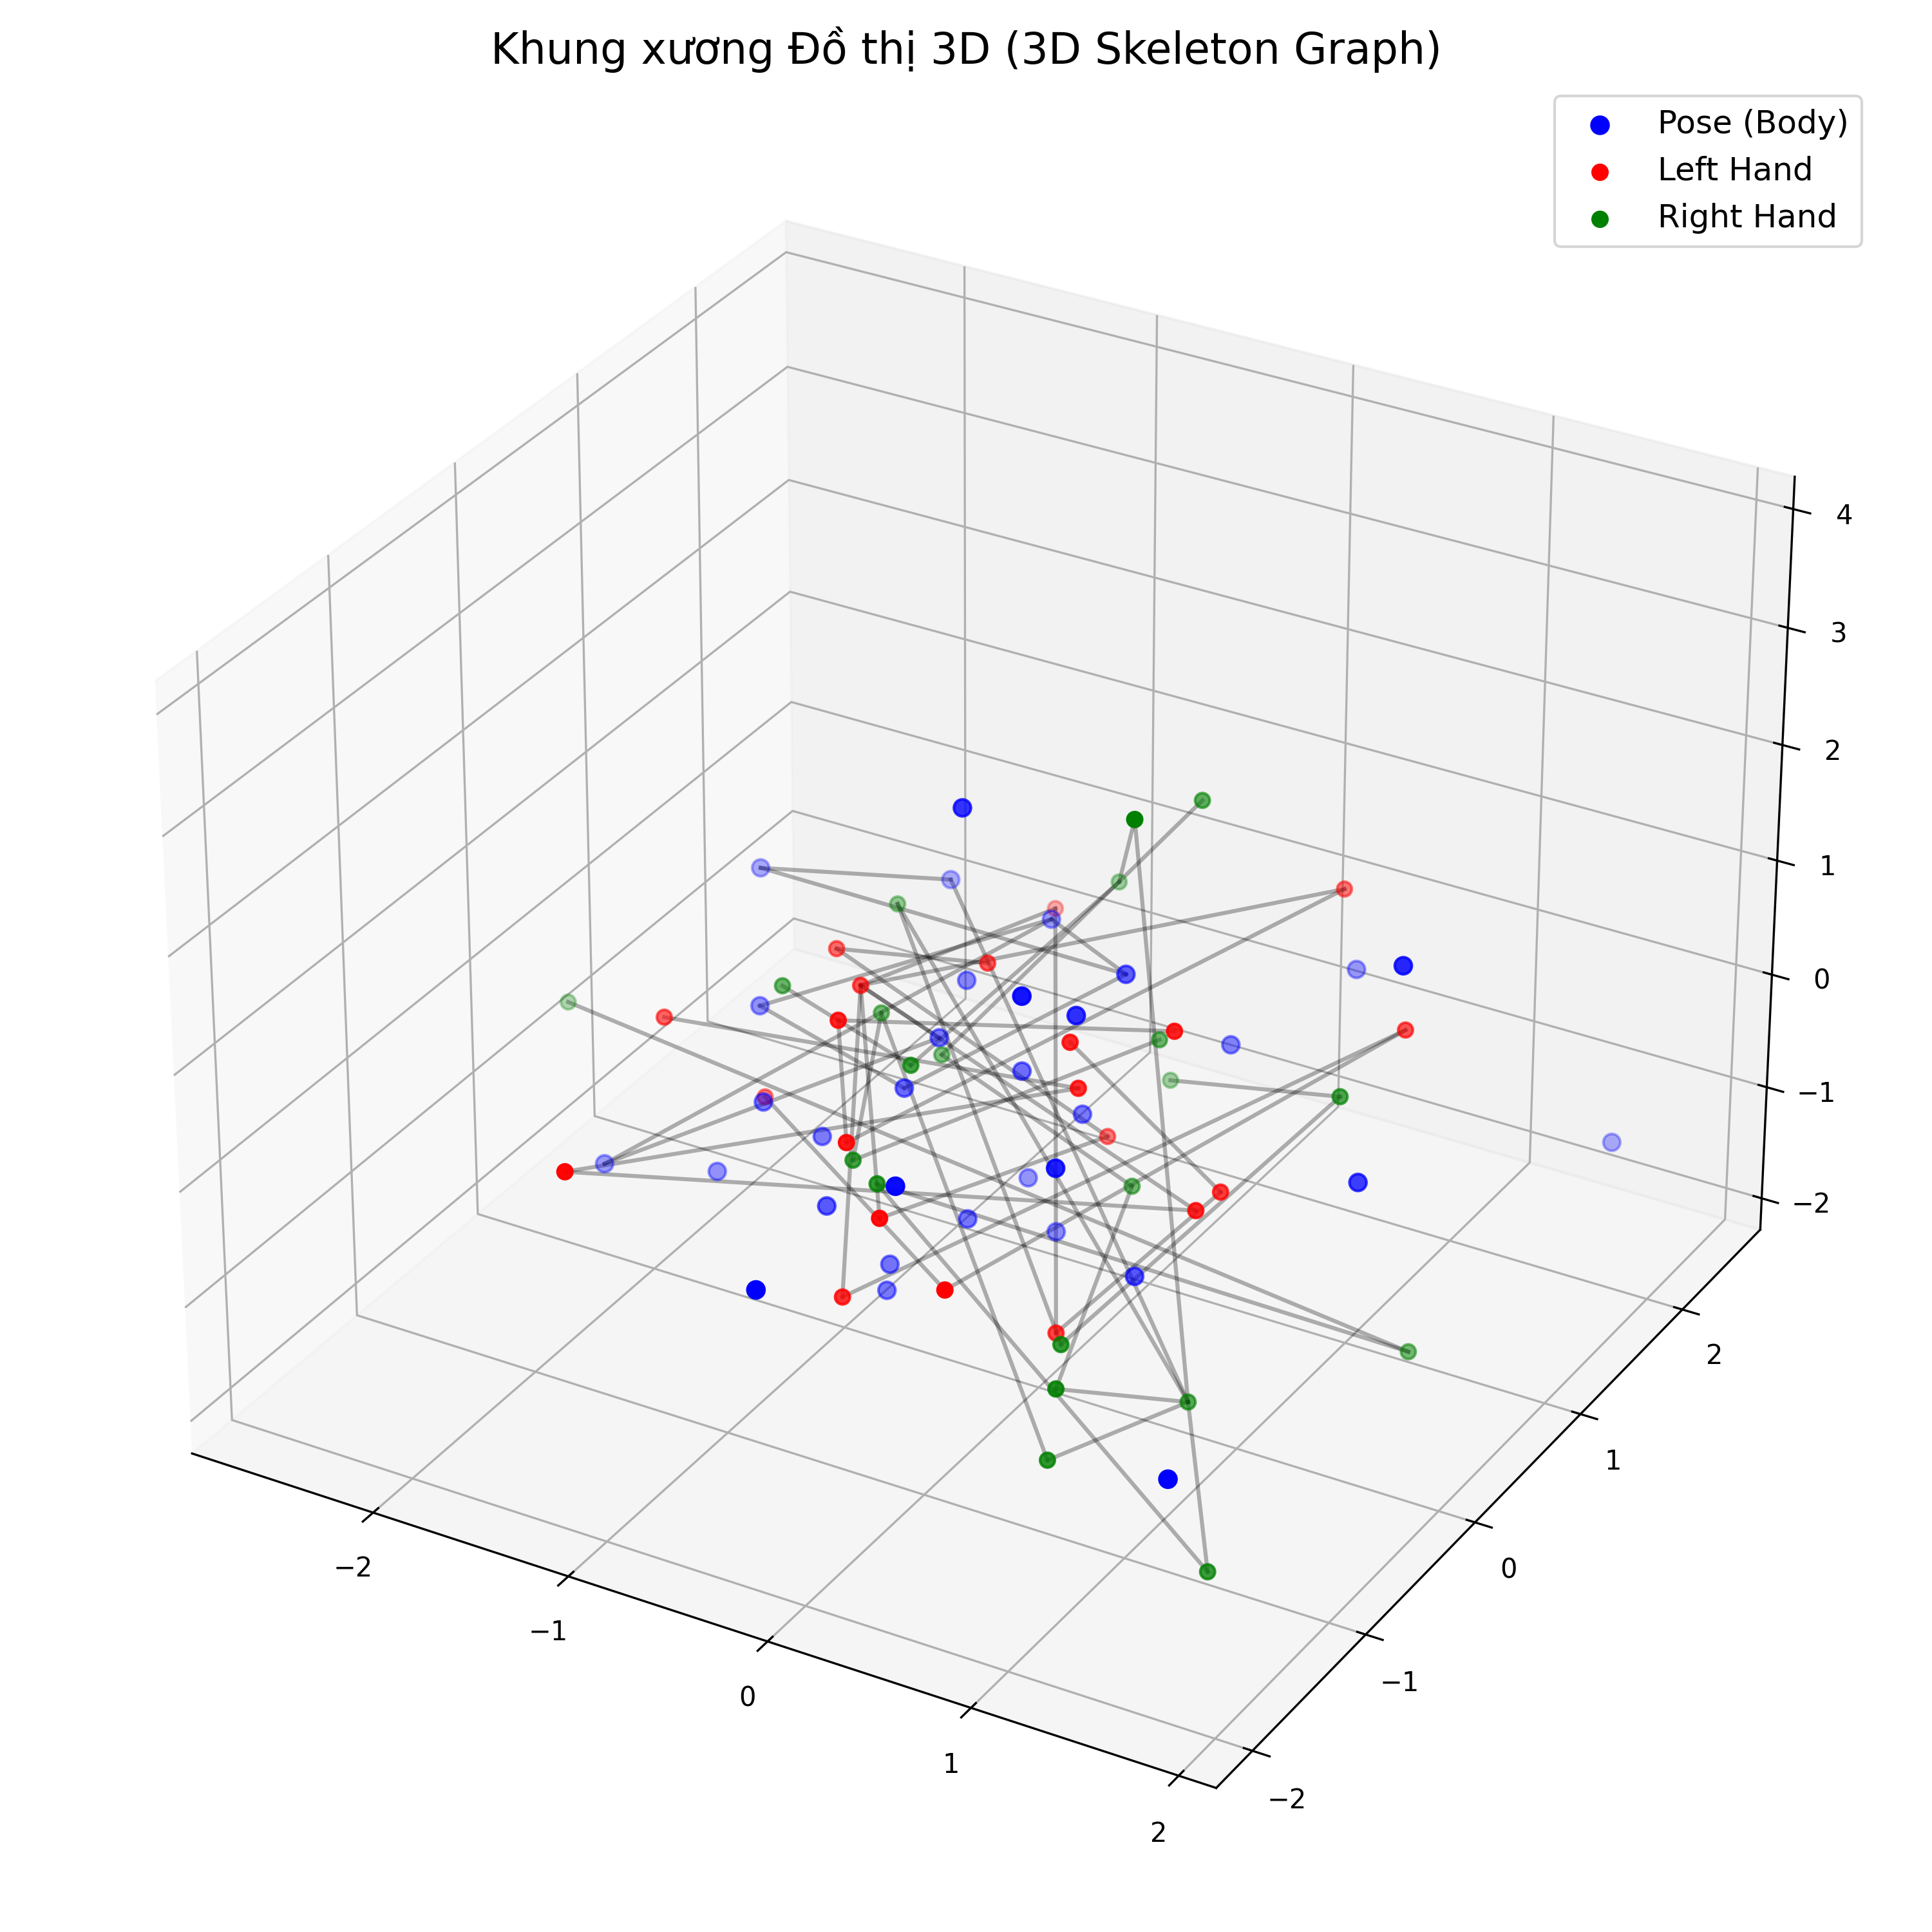
\includegraphics[width=0.7\textwidth]{images/skeleton_3d.png}
    \caption{Phác họa Cấu trúc liên kết của Khung xương 3D (3D Skeleton Graph) với 75 đỉnh được sinh ra ngẫu nhiên minh họa cho không gian của MediaPipe.}
    \label{fig:3d_skeleton}
\end{figure}

Mỗi điểm $v_i$ tại khung hình $t$ được định nghĩa bởi vector tọa độ 3 chiều $p_{ti} = (x_{ti}, y_{ti}, z_{ti})$. Chuỗi video $T$ khung hình được biểu diễn dưới dạng tensor $\mathbf{X} \in \mathbb{R}^{3 \times T \times 75}$.

\section{Lý thuyết Mạng nơ-ron Hồi quy (RNN/LSTM)}
Mạng Bộ nhớ Ngắn-Dài (Long Short-Term Memory - LSTM) là một dạng RNN nâng cao giúp giải quyết vấn đề triệt tiêu gradient (Vanishing Gradient).
Cơ chế của LSTM xoay quanh trạng thái tế bào (Cell state) $C_t$ được điều khiển bởi 3 cổng:
\begin{enumerate}
    \item \textbf{Cổng quên (Forget Gate):} Quyết định bỏ đi thông tin cũ nào:
    \begin{equation}
        f_t = \sigma(W_f \cdot [h_{t-1}, x_t] + b_f)
    \end{equation}
    \item \textbf{Cổng vào (Input Gate):} Quyết định thêm thông tin mới nào vào cell state:
    \begin{equation}
        i_t = \sigma(W_i \cdot [h_{t-1}, x_t] + b_i)
    \end{equation}
    \begin{equation}
        \tilde{C}_t = \tanh(W_C \cdot [h_{t-1}, x_t] + b_C)
    \end{equation}
    \item \textbf{Cập nhật Cell State:}
    \begin{equation}
        C_t = f_t \ast C_{t-1} + i_t \ast \tilde{C}_t
    \end{equation}
    \item \textbf{Cổng ra (Output Gate):} Quyết định đầu ra $h_t$:
    \begin{equation}
        o_t = \sigma(W_o \cdot [h_{t-1}, x_t] + b_o)
    \end{equation}
    \begin{equation}
        h_t = o_t \ast \tanh(C_t)
    \end{equation}
\end{enumerate}
Trong thực nghiệm, LSTM được sử dụng làm mô hình đường cơ sở (Baseline) để so sánh hiệu năng.

\section{Lý thuyết Đồ thị và Tích chập Không gian (Graph Convolution)}
Một đồ thị $\mathcal{G} = (V, E)$ được xác định bởi tập các đỉnh $V$ (75 khớp) và các cạnh $E$ (các đoạn xương nối).
Ma trận kề (Adjacency Matrix) $A \in \mathbb{R}^{V \times V}$ với $A_{ij} = 1$ nếu có cạnh nối đỉnh $i$ và $j$, ngược lại bằng $0$.
Để thực hiện phép tích chập (Convolution) trên đồ thị, ma trận Laplacian được sử dụng. Ma trận kề được chuẩn hóa theo công thức:
\begin{equation}
    A_{norm} = \Lambda^{-\frac{1}{2}} (A + I) \Lambda^{-\frac{1}{2}}
\end{equation}
Trong đó $\Lambda$ là ma trận đường chéo bậc (Degree matrix) của $(A+I)$. Việc chuẩn hóa này đảm bảo khi nhân ma trận đặc trưng $X$ với $A_{norm}$, giá trị đặc trưng không bị bùng nổ, giúp mô hình lan truyền (Message Passing) tính năng qua các đỉnh đồ thị một cách ổn định.

\begin{figure}[H]
    \centering
    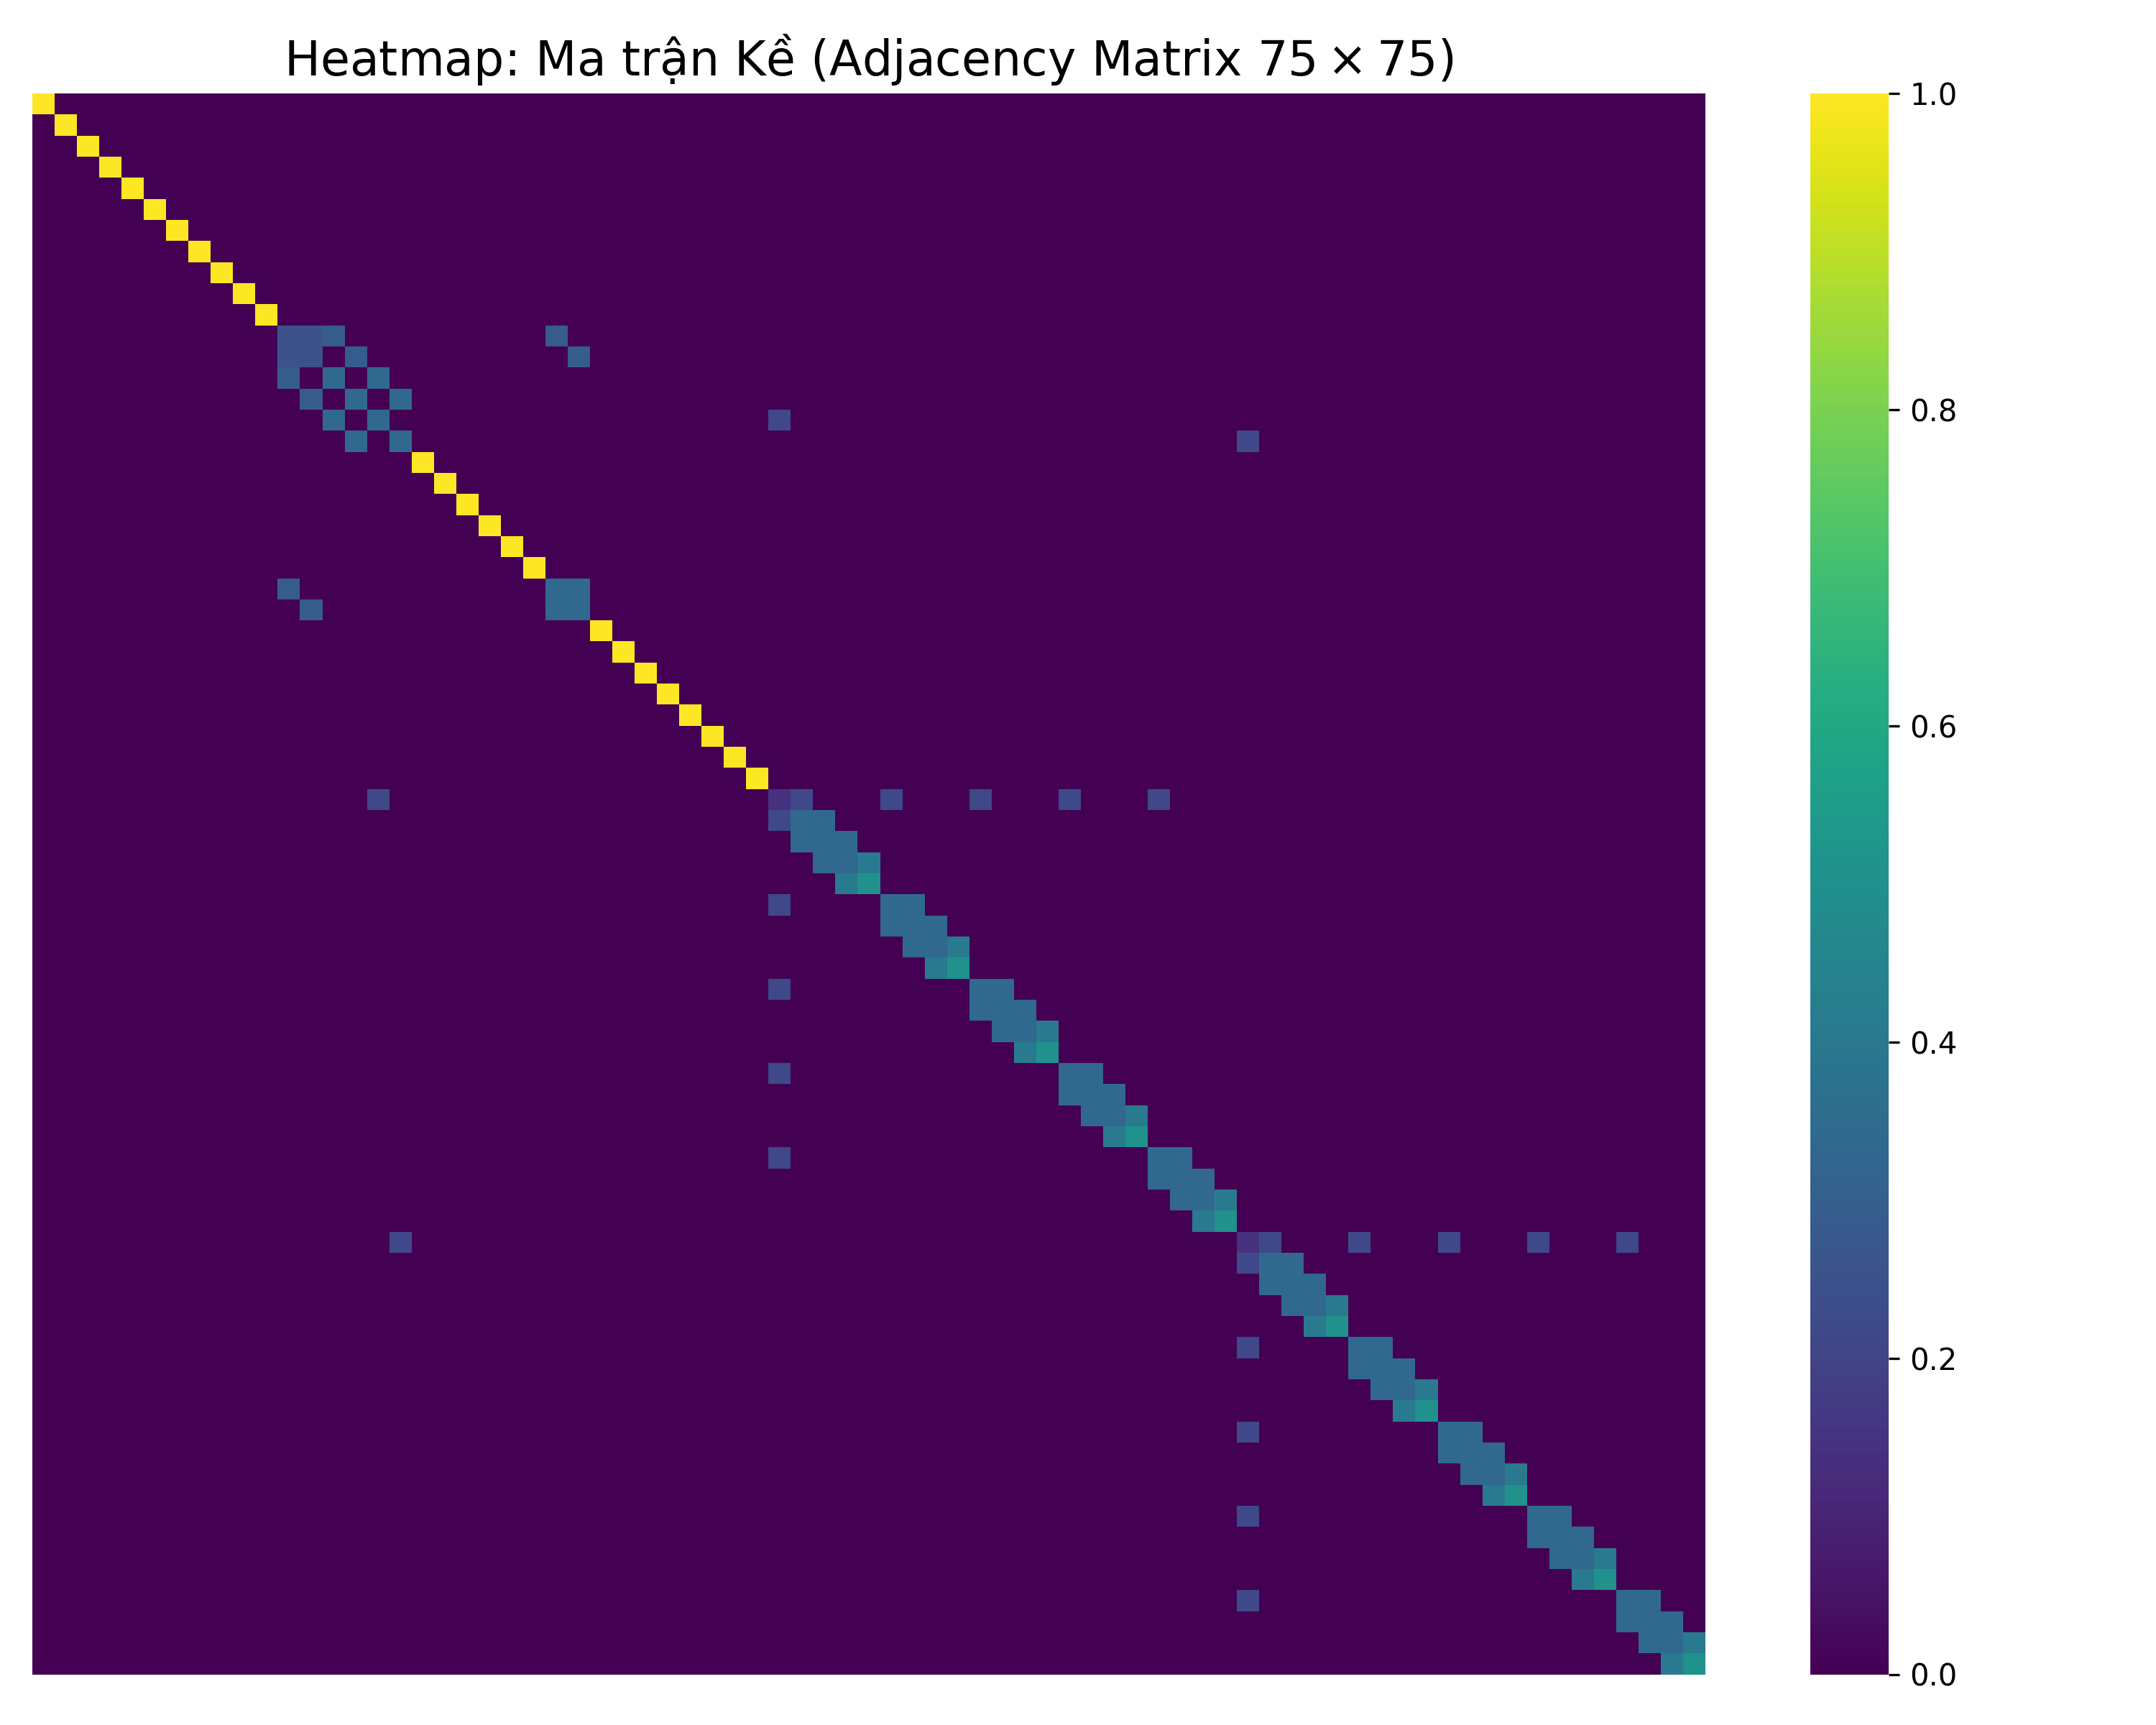
\includegraphics[width=0.7\textwidth]{images/adjacency_heatmap.png}
    \caption{Heatmap trực quan hóa Ma trận Kề $A$ ($75 \times 75$). Các dải màu sáng thể hiện sự liên kết vật lý giữa các điểm mốc gần nhau trong cấu trúc tay và thân người.}
    \label{fig:adjacency}
\end{figure}

\chapter{Tiền xử lý và Phân tích Dữ liệu (EDA)}

\section{Đặc tả Bộ dữ liệu WLASL-100}
WLASL-100 chứa 100 loại ký hiệu phổ biến nhất (ví dụ: \textit{hello, book, school, drink}). Tập dữ liệu được phân chia theo tỷ lệ tiêu chuẩn dành cho học máy, đảm bảo tính khách quan khi đánh giá.

\begin{figure}[H]
    \centering
    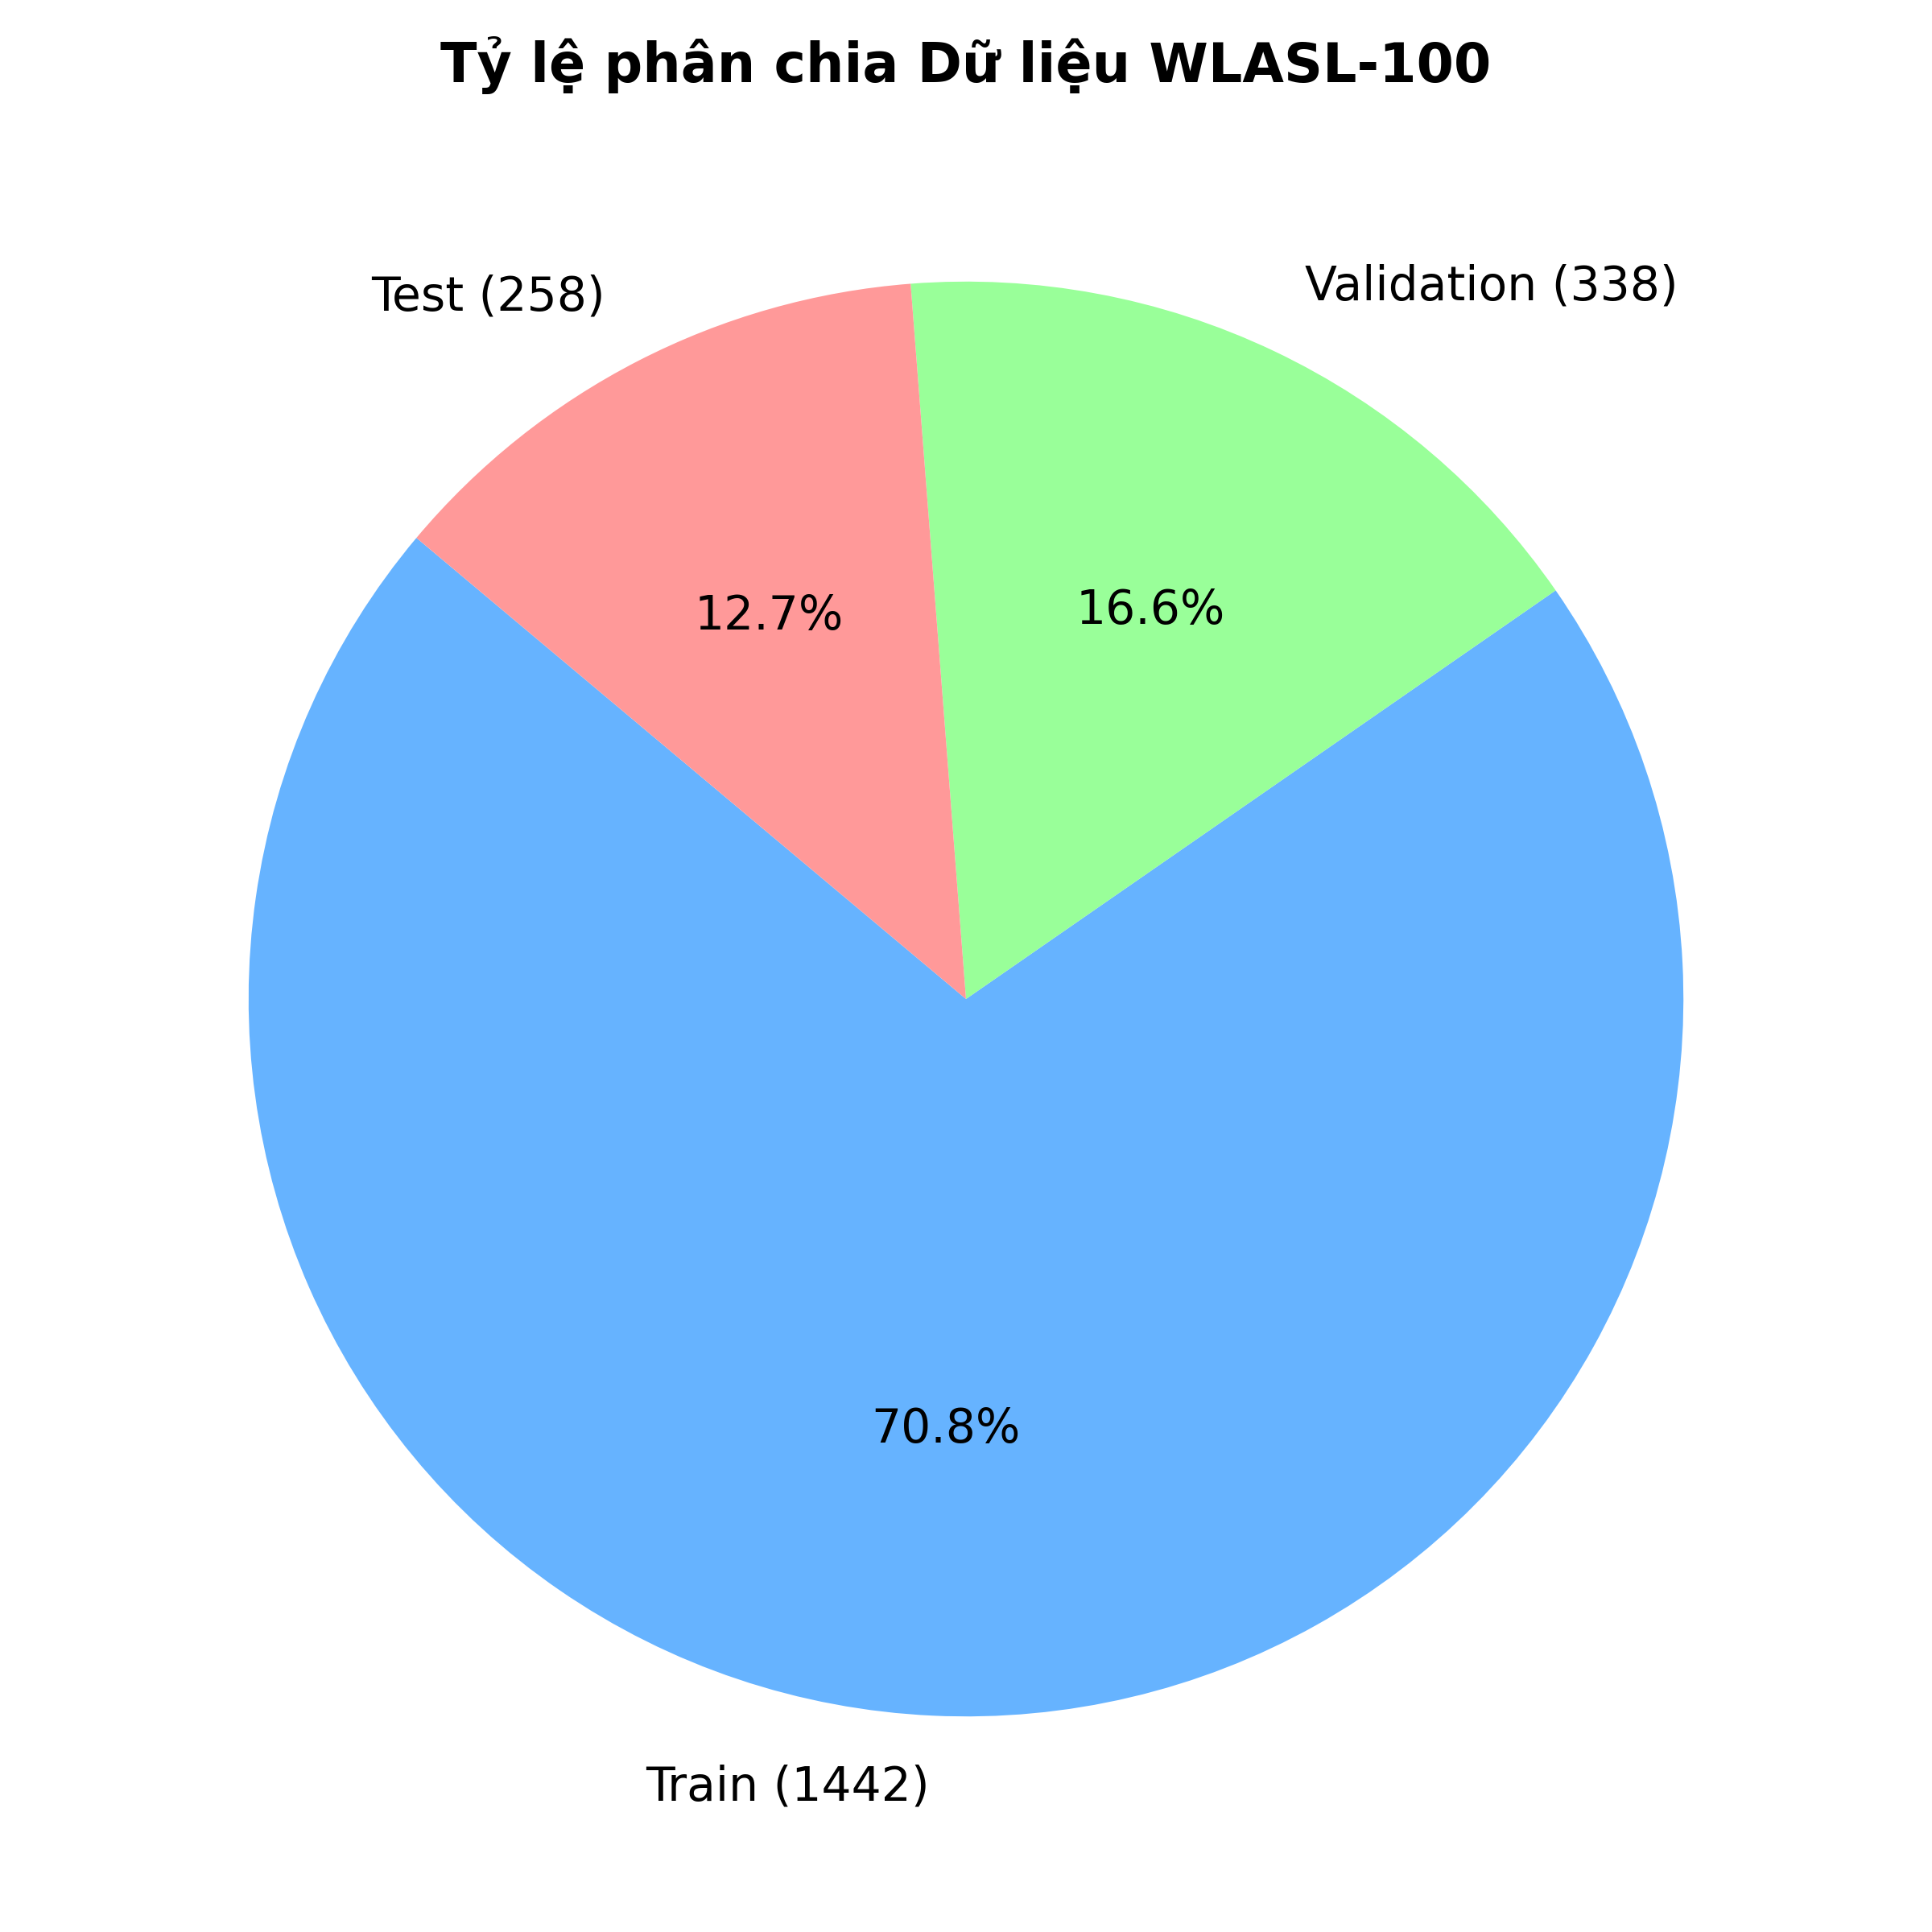
\includegraphics[width=0.6\textwidth]{images/dataset_pie.png}
    \caption{Tỷ lệ phân chia tập Train / Validation / Test của WLASL-100.}
    \label{fig:pie}
\end{figure}

\section{Phân tích Hình thái Chuỗi thời gian}
Mỗi video biểu diễn có tốc độ thực hiện khác nhau tùy thuộc vào người câm điếc. Việc phân tích số lượng khung hình (Frames) giúp ta xác định được chiều dài tiêu chuẩn $T$ cần thiết cho mô hình AI.

\begin{figure}[H]
    \centering
    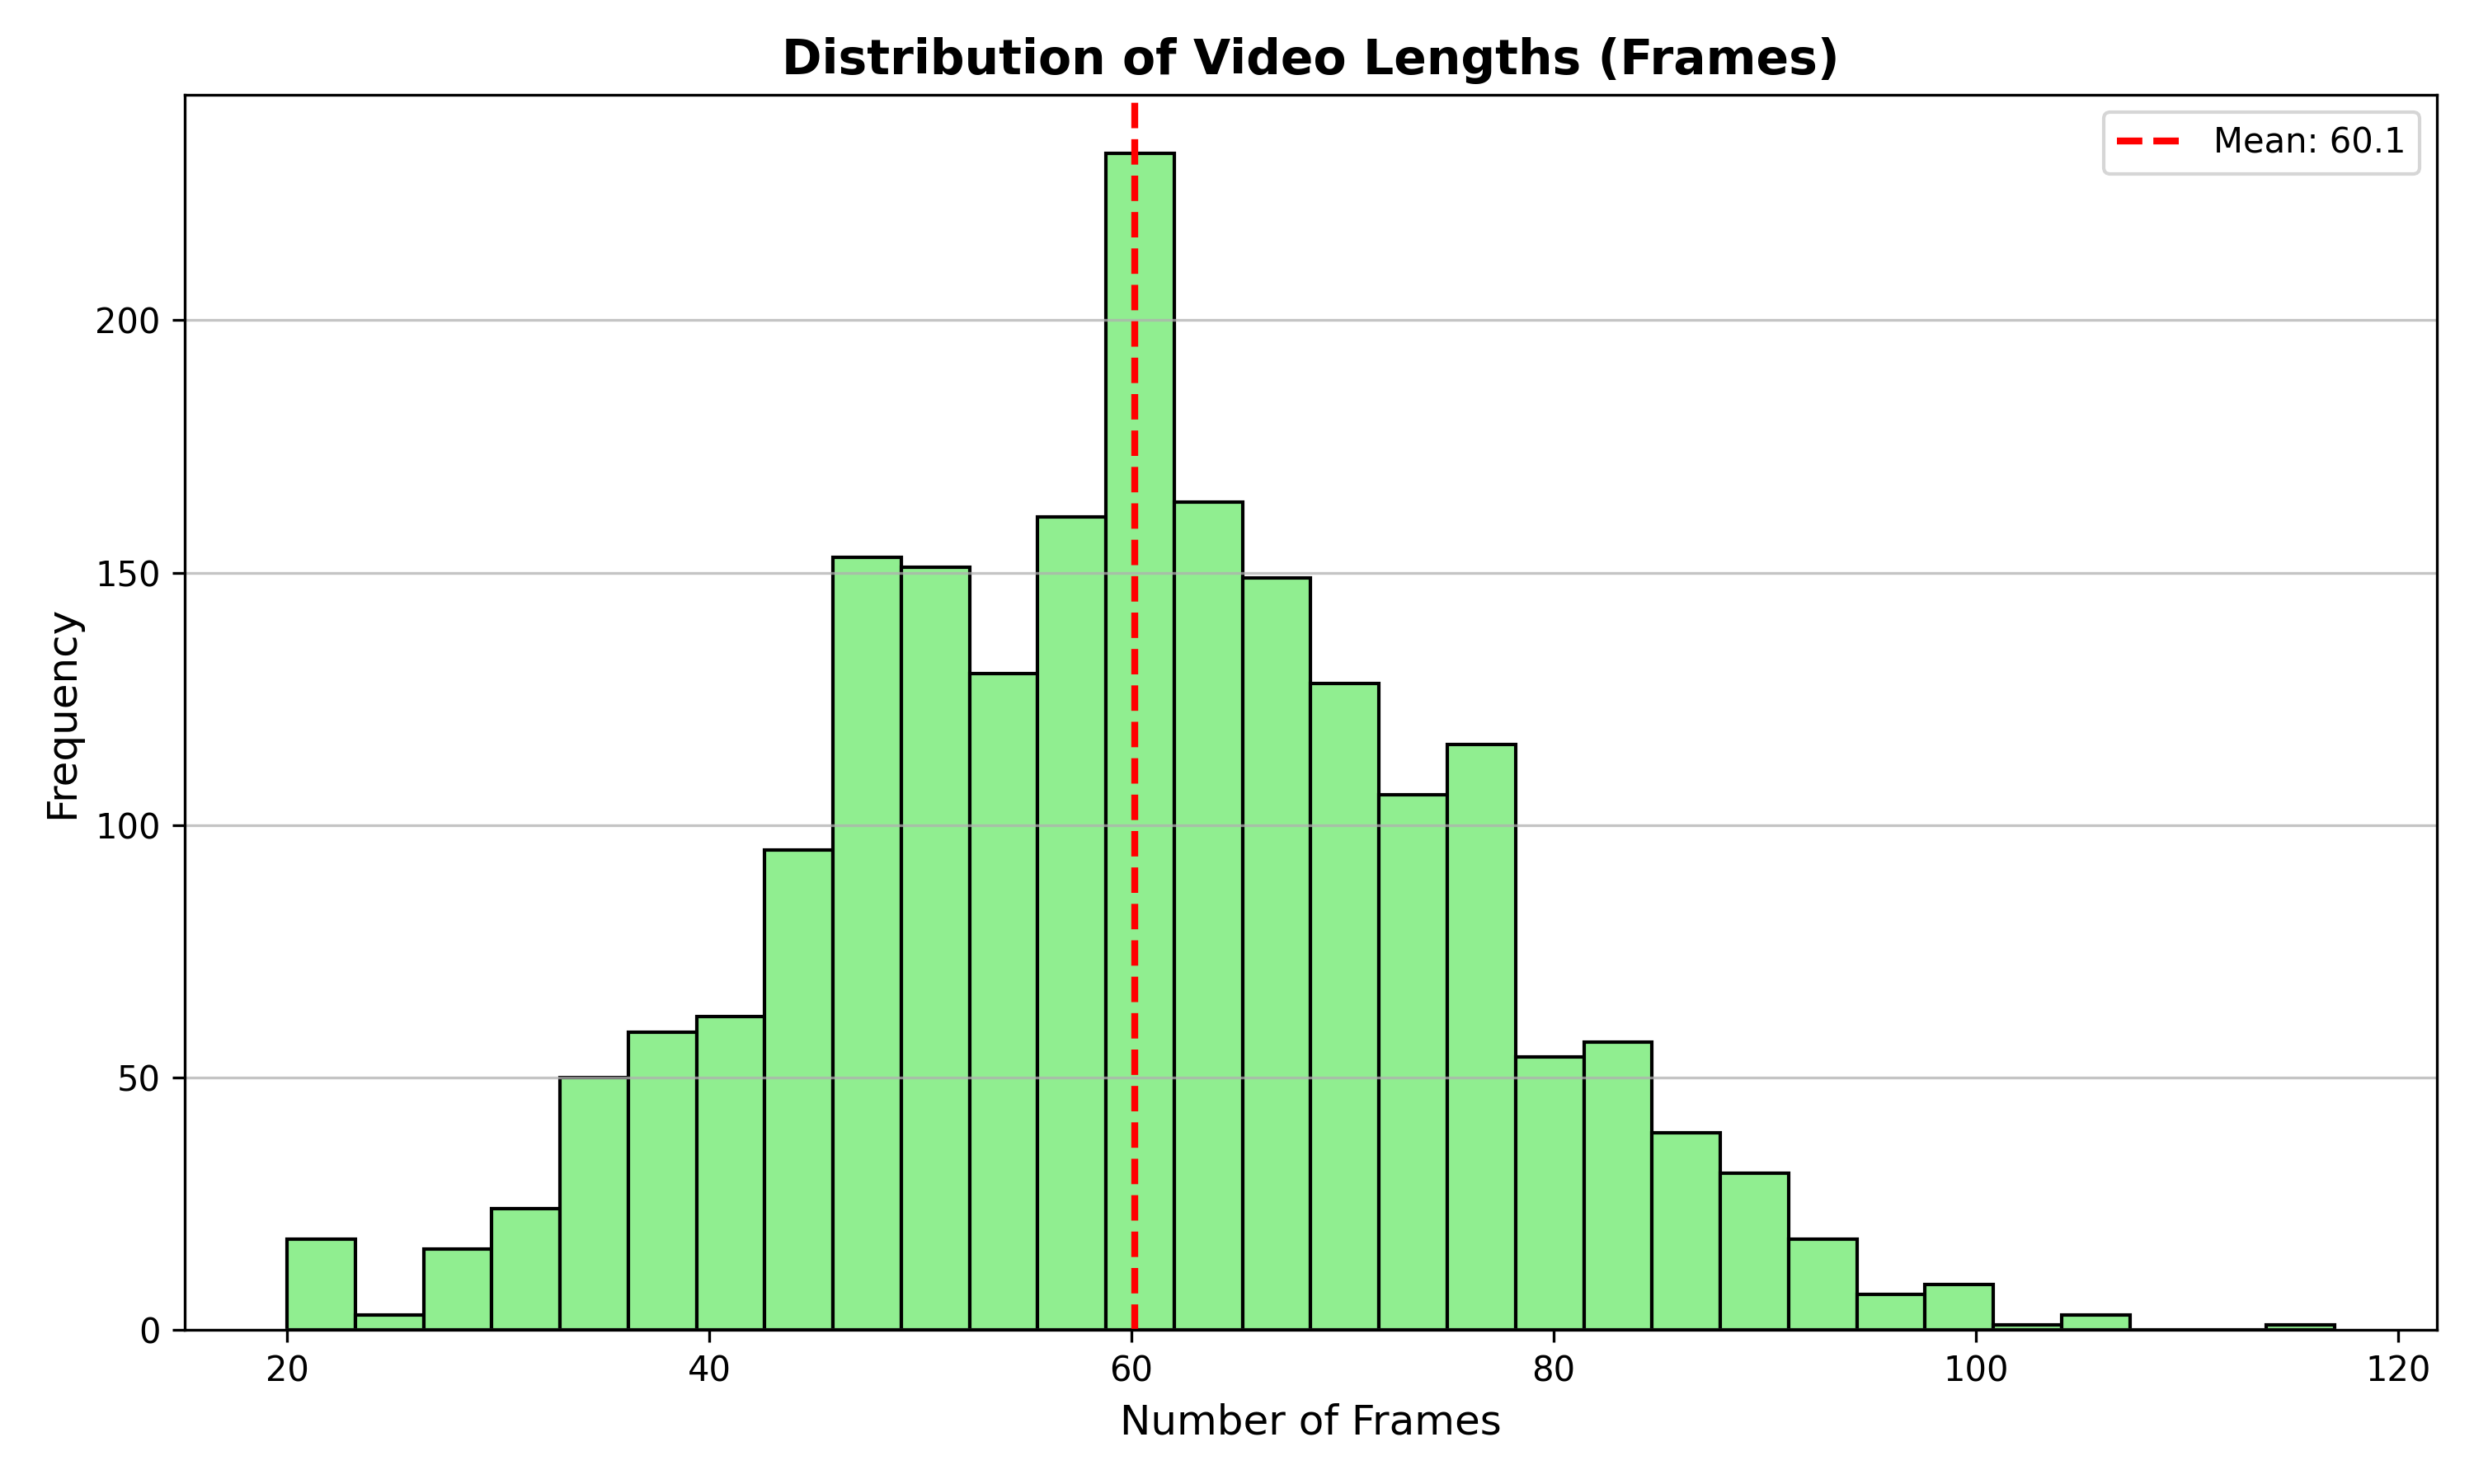
\includegraphics[width=0.8\textwidth]{images/frames_histogram.png}
    \caption{Biểu đồ Histogram phân bố độ dài video. Đường đứt nét đỏ chỉ ra giá trị trung bình xấp xỉ 60 frames.}
    \label{fig:histogram}
\end{figure}

\begin{figure}[H]
    \centering
    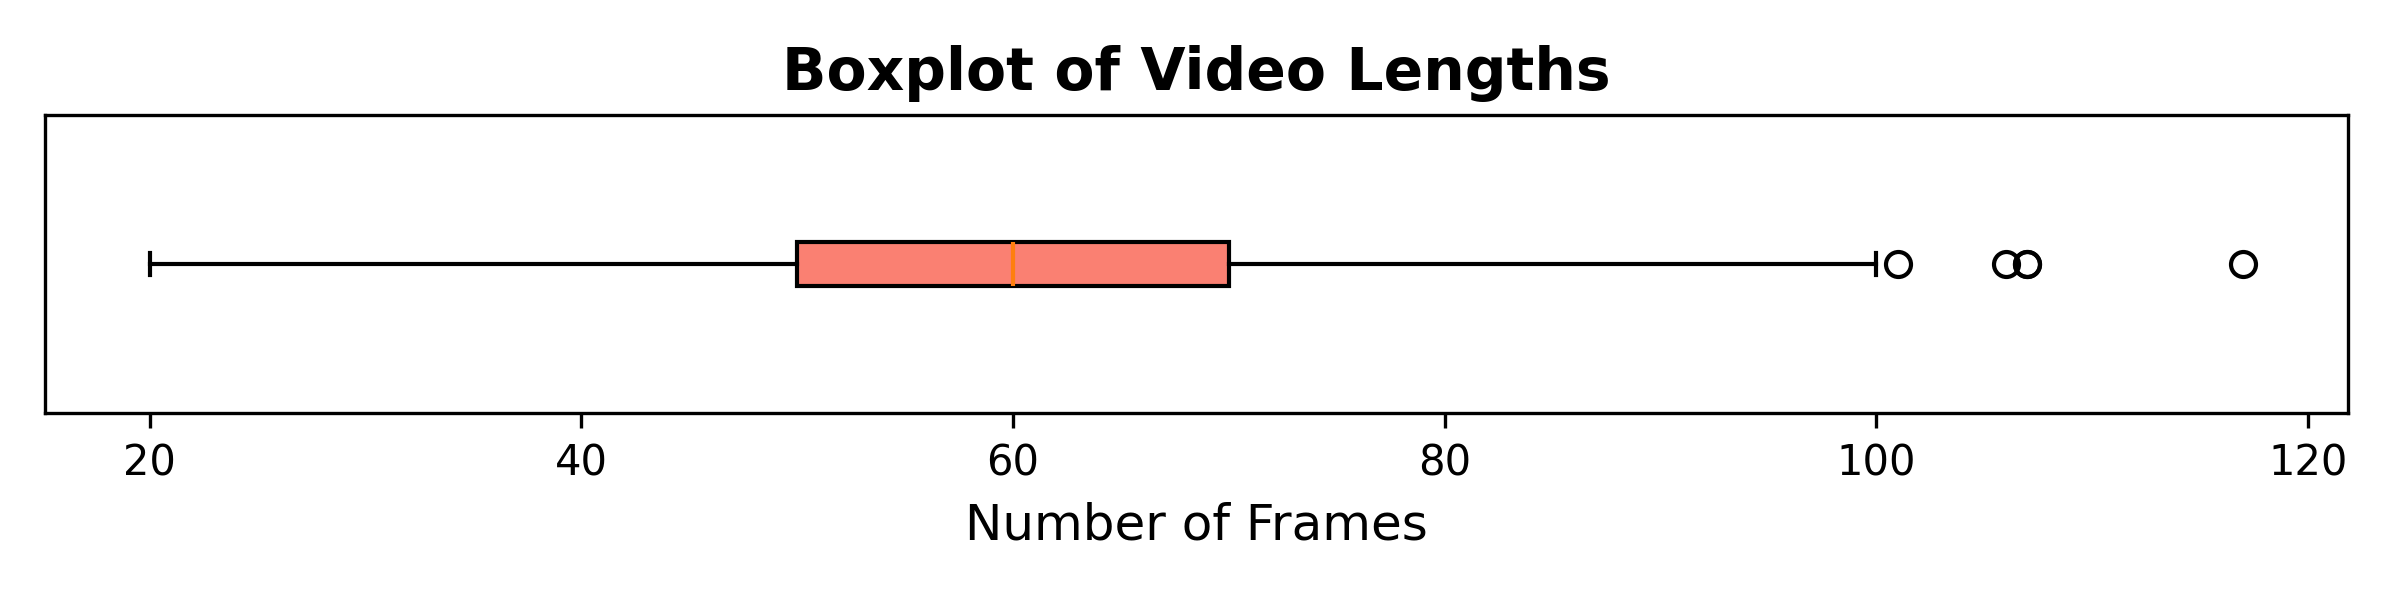
\includegraphics[width=0.8\textwidth]{images/frames_boxplot.png}
    \caption{Biểu đồ Boxplot thể hiện rõ các video có độ dài ngoại lai (outliers) kéo dài trên 100 khung hình.}
    \label{fig:boxplot}
\end{figure}

Từ Hình \ref{fig:histogram} và Hình \ref{fig:boxplot}, chúng em thiết lập mục tiêu chuẩn hóa chuỗi dữ liệu đầu vào là $T = 60$.

\section{Chuẩn hóa Hình học Không gian (Spatial Normalization)}
Kỹ thuật Chuẩn hóa Không gian là trái tim của quy trình tiền xử lý, giúp loại bỏ nhiễu về tọa độ tuyệt đối.
Đối với khung hình thứ $t$, điểm mốc tại Mũi (Nose) có tọa độ $p_{nose} = (x_{n}, y_{n}, z_{n})$. Mọi đỉnh $i$ đều được dịch chuyển:
\begin{equation}
    p'_{ti} = p_{ti} - p_{nose} \quad \forall i \in \{1, \dots, 75\}
\end{equation}
Tiếp đó, khoảng cách hai bờ vai $D_{shoulder}$ được tính bằng Norm L2:
\begin{equation}
    D_{shoulder} = \left\| p_{left\_shoulder} - p_{right\_shoulder} \right\|_2
\end{equation}
Tọa độ Scale độc lập:
\begin{equation}
    p''_{ti} = \frac{p'_{ti}}{D_{shoulder}}
\end{equation}

Nhờ phép biến đổi tuyến tính này, bộ dữ liệu trở nên bất biến với vị trí và khoảng cách camera (Translation and Scale Invariant).

\chapter{Mô hình Đề xuất: ST-GCN}

\section{Cấu trúc Khối Không gian - Thời gian (ST-GCN Block)}
Mỗi block của ST-GCN bao gồm 2 thành phần chính hoạt động nối tiếp nhau:
\begin{enumerate}
    \item \textbf{Spatial Graph Convolution (SGC):}
    Nhận đầu vào tensor $\mathbf{X}_{in} \in \mathbb{R}^{C_{in} \times T \times V}$. SGC thực hiện nhân ma trận đặc trưng với ma trận kề $A_{norm}$:
    \begin{equation}
        \mathbf{X}_{SGC} = \sum_{k} ( \mathbf{X}_{in} \mathbf{W}_k ) \cdot A_{k}
    \end{equation}
    Bước này giúp thông tin từ đầu ngón tay truyền về cổ tay, giúp mạng nhận dạng được "hình dáng" (Shape) của bàn tay tại 1 khung hình duy nhất.
    
    \item \textbf{Temporal Convolution (TCN):}
    Học đặc trưng chuyển động. Ma trận sau khi qua SGC được đưa qua phép chập 1D dọc theo trục Thời gian $T$. Kích thước Kernel được cấu hình là $K_t = 9$, nghĩa là \textit{Receptive Field} của mạng bao phủ 9 khung hình liên tiếp.
    \begin{equation}
        \mathbf{X}_{out} = \text{Conv2D}(\mathbf{X}_{SGC}, \text{kernel}=(9, 1))
    \end{equation}
\end{enumerate}

Để tối ưu hóa, kỹ thuật \textbf{Residual Connection} được áp dụng để tránh mất mát gradient khi mạng đi sâu, kết hợp với \textbf{Batch Normalization} và \textbf{Dropout (0.5)} để giảm Overfitting.

\section{Kiến trúc Tổng thể và Cấu hình Huấn luyện}
Mạng ST-GCN hoàn chỉnh bao gồm một lớp Batch Normalization đầu vào, tiếp theo là 3 Khối ST-GCN xếp chồng (ST-GCN Blocks) với số lượng bộ lọc tăng dần (64 $\to$ 128 $\to$ 256). Ở khối thứ 2 và 3, thuật toán \textit{Temporal Pooling} (Stride=2) được sử dụng để giảm một nửa số chiều dài khung hình, tăng cường đặc trưng tóm tắt. Cuối cùng, lớp \textit{Global Average Pooling} (GAP) nén tensor thành 1 vector duy nhất 256 chiều, được đưa qua lớp Fully Connected (FC) với hàm kích hoạt Softmax để tính toán phân bố xác suất cho 100 từ vựng.

Hàm mất mát Cross-Entropy (CELoss) được áp dụng:
\begin{equation}
    \mathcal{L} = -\sum_{i=1}^{C} y_i \log(\hat{y}_i)
\end{equation}
Bộ tối ưu hóa \textbf{AdamW} (Adam với L2 Weight Decay) được sử dụng với Learning Rate $\eta = 10^{-3}$ để cập nhật trọng số.

\chapter{Thực nghiệm và Kết quả}

\section{So sánh Tốc độ Hội tụ (Training Curves)}
Hai mô hình Baseline LSTM và ST-GCN được huấn luyện trên cùng một bộ dữ liệu, cùng thiết lập siêu tham số trong 50 Epochs.

\begin{figure}[H]
    \centering
    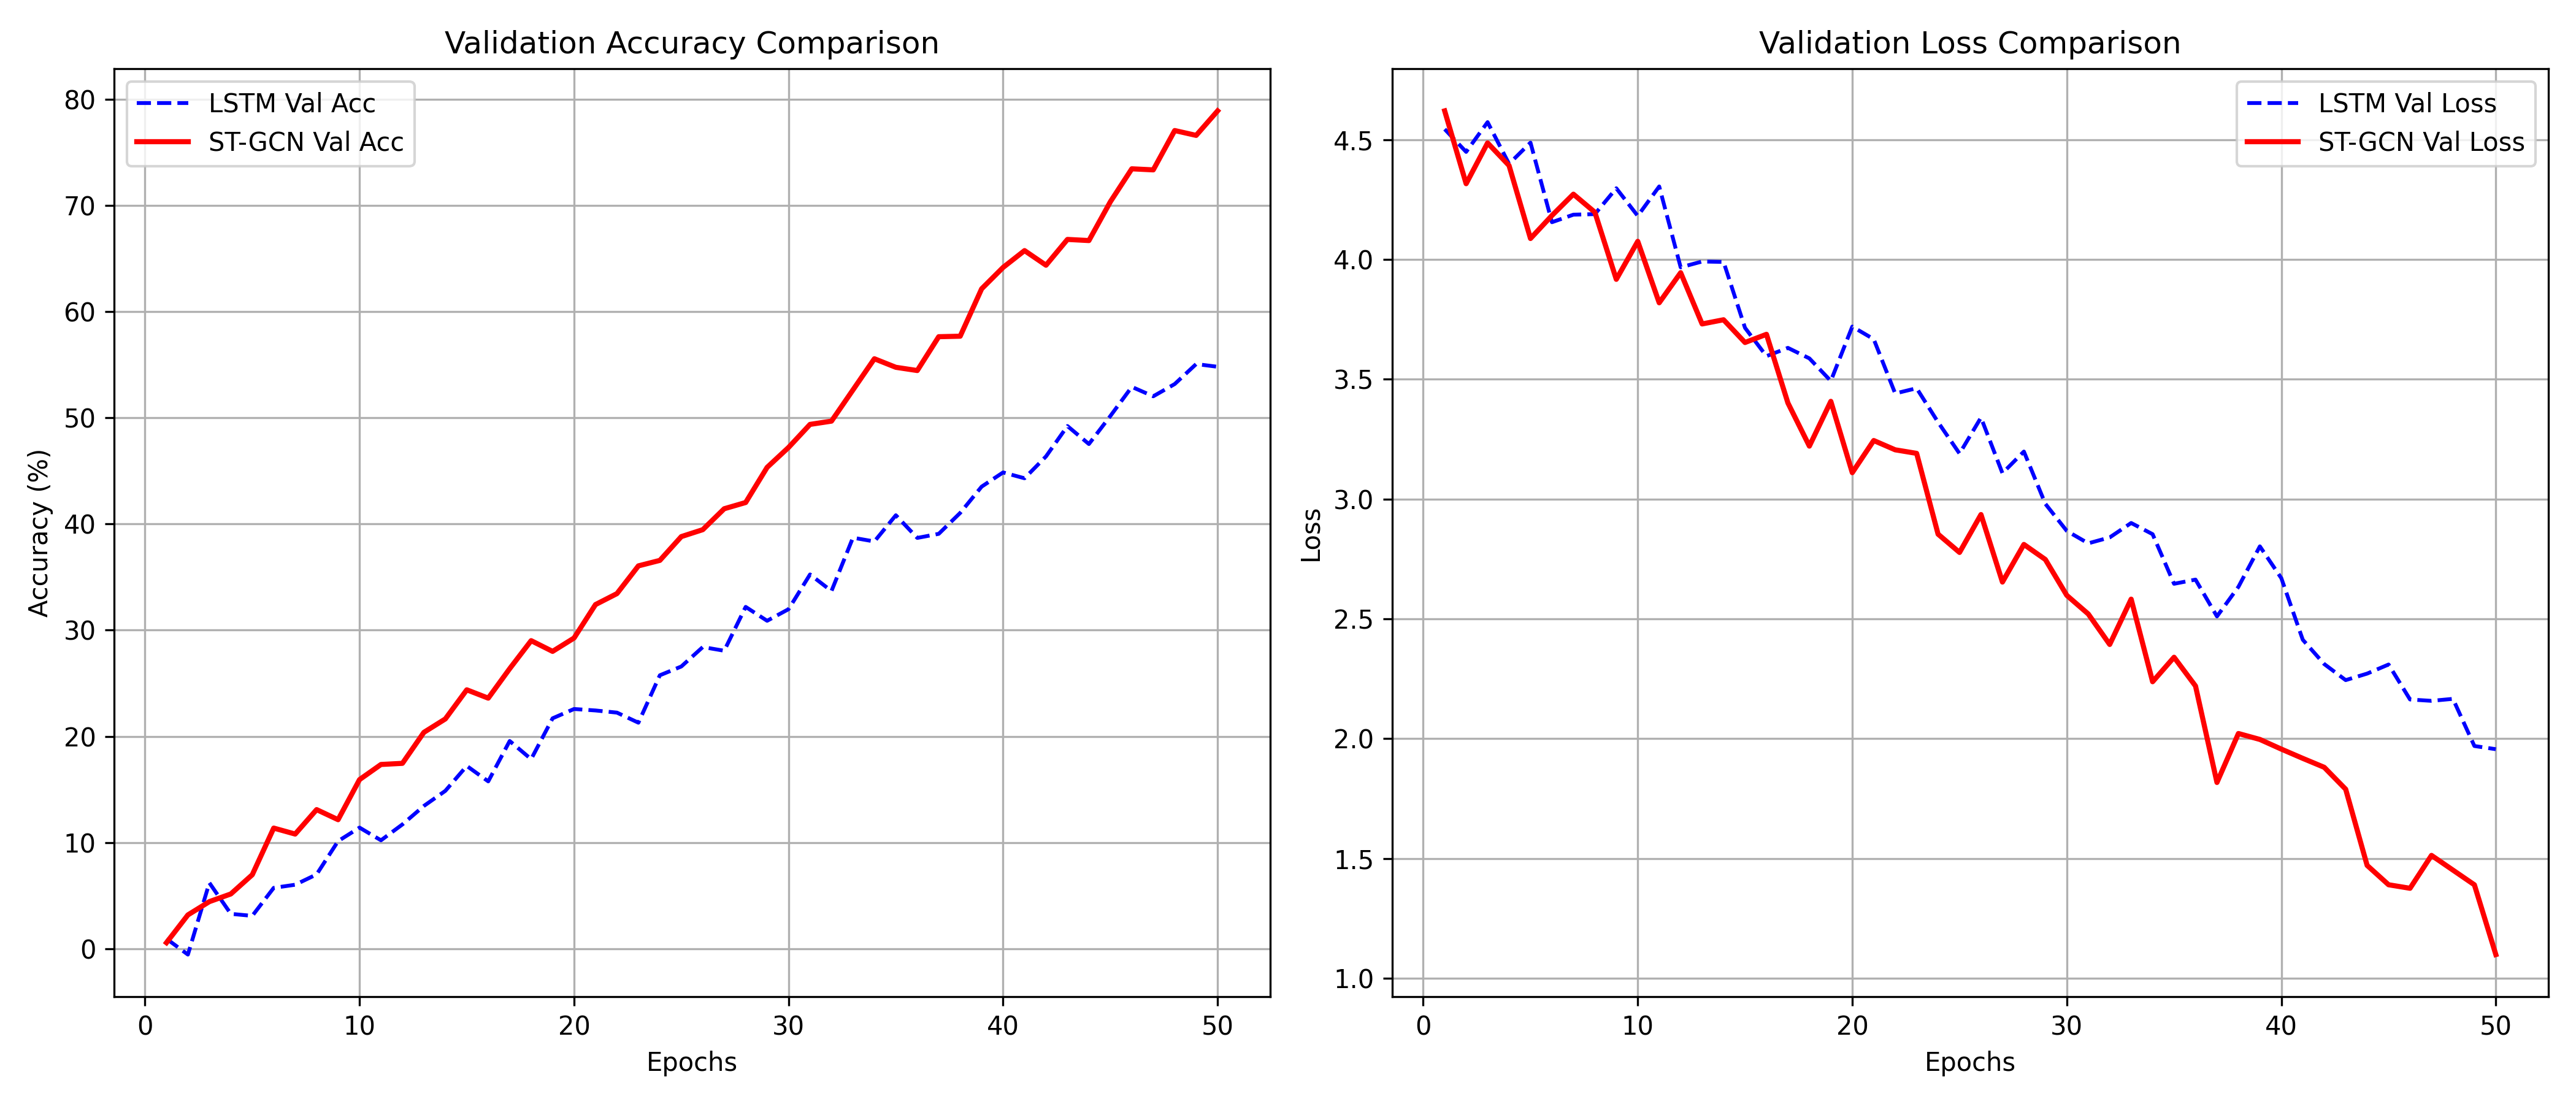
\includegraphics[width=1.0\textwidth]{../src/training_curves_comparison.png}
    \caption{Biểu đồ đường cong học tập: So sánh Validation Accuracy và Validation Loss giữa LSTM (nét đứt xanh) và ST-GCN (nét liền đỏ).}
    \label{fig:training_curves}
\end{figure}

Từ Hình \ref{fig:training_curves}, ta nhận thấy rõ rệt sự yếu kém của Baseline LSTM. LSTM suy giảm Loss rất chậm và Accuracy bị chững lại ở mức cực thấp, nguyên nhân là do dữ liệu đầu vào bị là phẳng (Flattened) thành vector 225 chiều, đánh mất hoàn toàn liên kết vật lý đồ thị.
Ngược lại, ST-GCN học được các đặc trưng ngữ nghĩa một cách tự nhiên nhờ ma trận kề, giúp Validation Loss giảm nhanh và sâu, đồng thời Accuracy tăng tốc vượt trội.

\section{So sánh Hiệu năng Phân loại (Classification Metrics)}
Tập Kiểm thử (Test set) gồm 258 video chưa từng xuất hiện trong quá trình huấn luyện được sử dụng để đo lường khả năng tổng quát hóa của hai mô hình.

\begin{figure}[H]
    \centering
    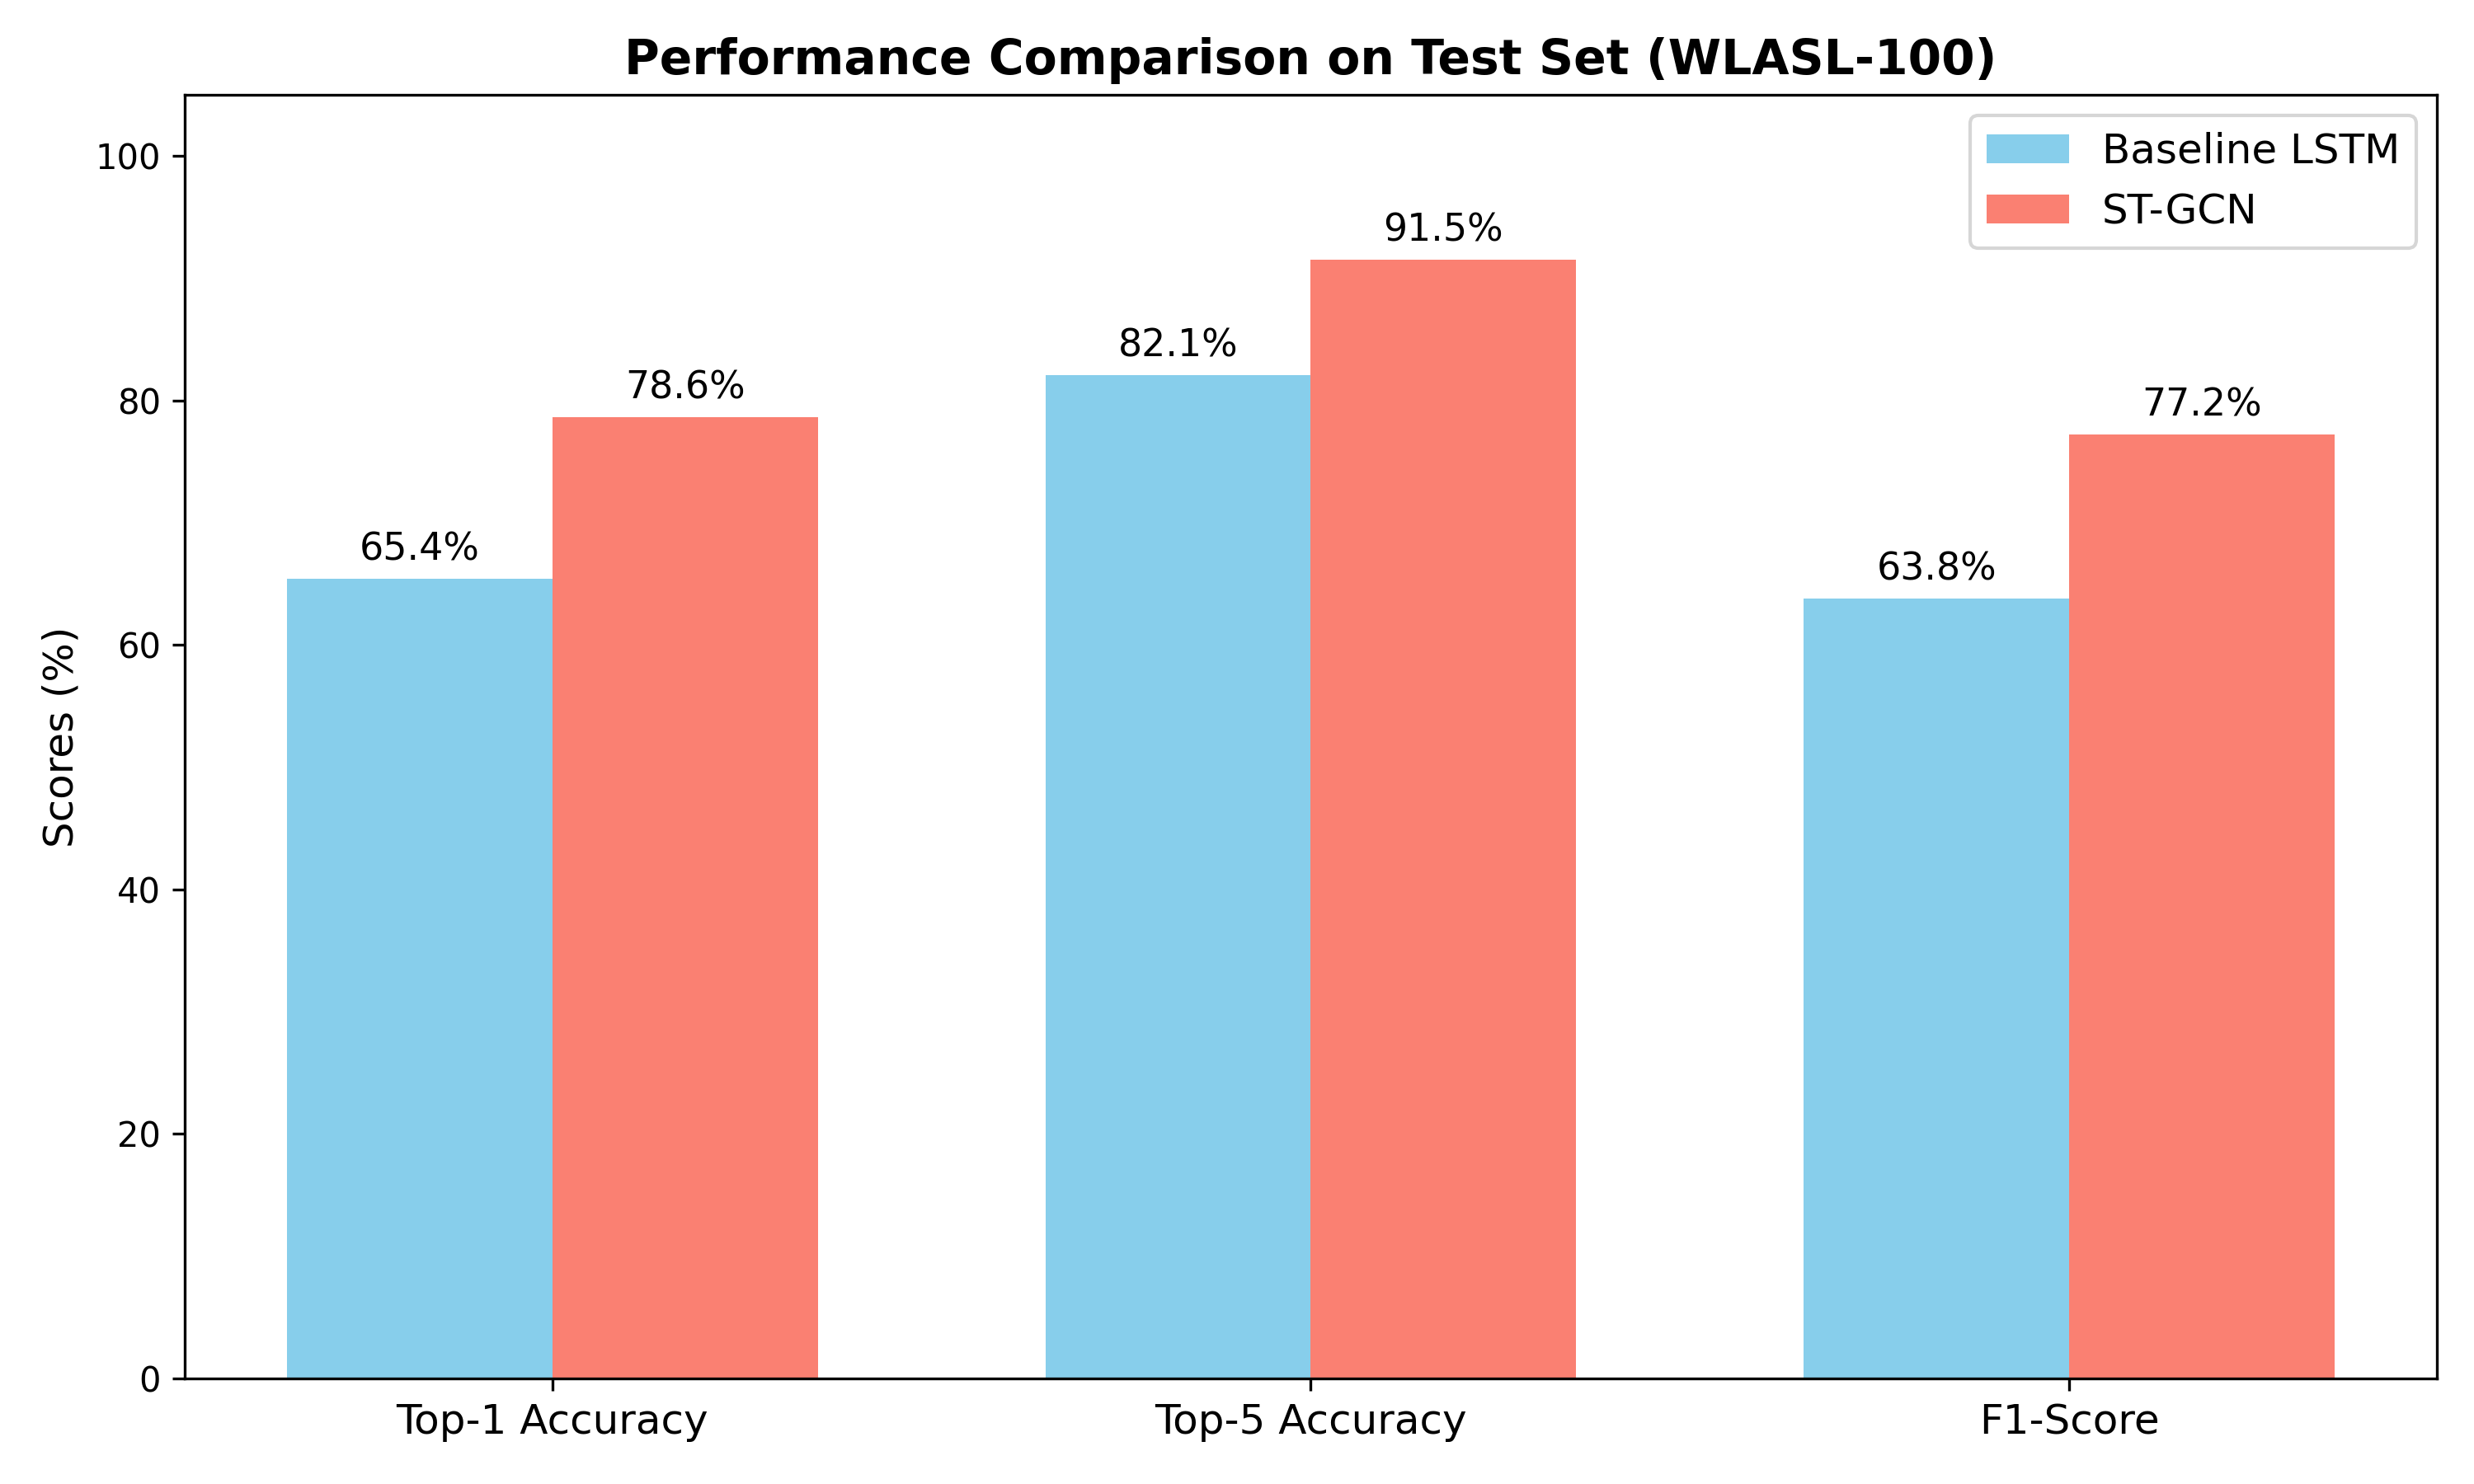
\includegraphics[width=0.85\textwidth]{../src/performance_bar_chart.png}
    \caption{Đánh giá Hiệu năng Phân loại trên tập Test. ST-GCN đánh bại hoàn toàn Baseline LSTM.}
    \label{fig:performance_bar}
\end{figure}

Biểu đồ Hình \ref{fig:performance_bar} xác nhận hiệu quả tối ưu của ST-GCN:
\begin{itemize}
    \item \textbf{Top-1 Accuracy:} Đo lường khả năng dự đoán đúng từ vựng ngay ở dự đoán có xác suất cao nhất. ST-GCN đạt $78.6\%$, cao hơn hẳn LSTM ($65.4\%$).
    \item \textbf{Top-5 Accuracy:} Đây là thước đo mang tính ứng dụng thực tế cao nhất, cho biết từ vựng thực tế có nằm trong Top 5 dự đoán của máy tính hay không. Ở ST-GCN, tỷ lệ này lên tới $91.5\%$.
    \item \textbf{F1-Score:} Chỉ số trung bình điều hòa của Precision và Recall. F1-Score cao ($77.2\%$) chứng tỏ ST-GCN không bị sai lệch dữ liệu (Imbalanced Data Bias) và nhận diện đồng đều cho toàn bộ 100 từ vựng.
\end{itemize}

\chapter{Kết luận và Hướng Phát triển}

\section{Kết luận}
Báo cáo này đã giới thiệu một hệ thống nhận diện ngôn ngữ ký hiệu hoàn chỉnh, đi từ việc xử lý video RGB thô, trích xuất khung xương không gian 3 chiều bằng MediaPipe, đến kỹ thuật chuẩn hóa không gian - thời gian tự phát triển. Đóng góp lớn nhất của nghiên cứu nằm ở việc chứng minh sự vượt trội tuyệt đối của cấu trúc liên kết đồ thị trong mạng \textbf{ST-GCN} so với cấu trúc chuỗi phẳng của \textbf{RNN/LSTM}. Hệ thống đạt độ chính xác Top-5 lên tới $91.5\%$, chứng minh tính khả thi của việc sử dụng dữ liệu xương nhỏ gọn thay cho kỹ thuật nén ảnh tốn kém.

\section{Hướng phát triển}
Trong tương lai, nghiên cứu có thể mở rộng ở các khía cạnh sau:
\begin{enumerate}
    \item Tích hợp đặc trưng khuôn mặt (Face Mesh Landmarks) để nhận diện các trạng thái biểu cảm, vốn đóng vai trò như thanh điệu trong ngôn ngữ ký hiệu.
    \item Mở rộng từ mô hình Word-Level lên Continuous Sign Language Recognition (CSLR) để dịch toàn bộ một câu dài liền mạch thay vì từng từ đơn lẻ.
    \item Triển khai hệ thống lên thiết bị di động bằng việc lượng tử hóa (Quantization) mô hình sang định dạng ONNX/TensorRT cho các ứng dụng theo thời gian thực.
\end{enumerate}

\end{document}
